% Chapter 9: Implementation Guide
\chapter{Implementation Guide}
\label{ch:implementation}

This chapter provides practical guidance for integrating \tprotocol{} into applications, with examples across all supported languages and frameworks.

\section{SDK Overview}
\label{sec:sdk-overview}

\tprotocol{} provides official SDKs for four major languages:

\begin{table}[ht]
\centering
\caption{Official SDK Comparison}
\label{tab:sdk-comparison}
\footnotesize
\begin{tabular}{l l l l l}
\toprule
\textbf{SDK} & \textbf{Version} & \textbf{Registry} & \textbf{Frameworks} & \textbf{License} \\
\midrule
TypeScript & 2.0.0 & npm @t402/* & Express, Fastify, Next.js & Apache 2.0 \\
Python & 1.7.1 & PyPI & FastAPI, Flask, Django & Apache 2.0 \\
Go & 1.5.0 & Go Modules & Gin, Echo, Chi & Apache 2.0 \\
Java & 1.1.0 & Maven Central & Spring Boot, WebFlux & Apache 2.0 \\
\bottomrule
\end{tabular}
\end{table}

\subsection{TypeScript SDK Architecture}

The TypeScript SDK is organized as a monorepo with 21 modular packages:

\begin{figure}[ht]
\centering
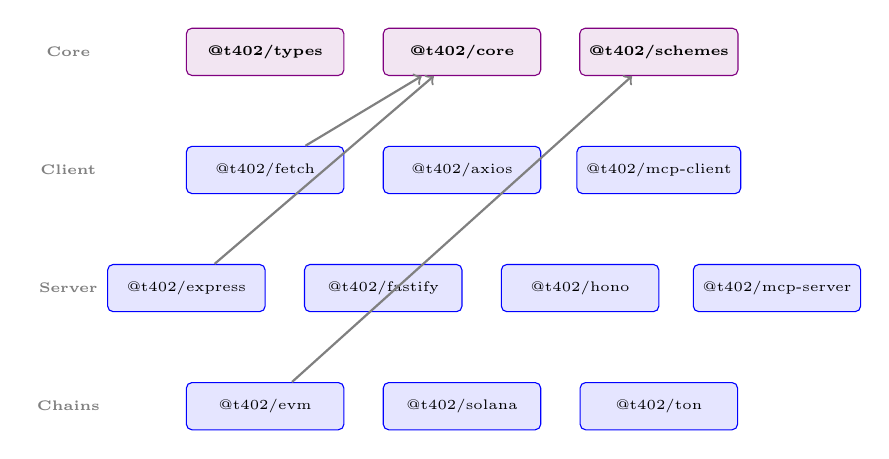
\begin{tikzpicture}[
    pkg/.style={
        rectangle,
        rounded corners=2pt,
        minimum width=2cm,
        minimum height=0.6cm,
        draw=blue,
        fill=blue!10,
        font=\tiny
    },
    core/.style={
        rectangle,
        rounded corners=2pt,
        minimum width=2cm,
        minimum height=0.6cm,
        draw=violet,
        fill=violet!10,
        font=\tiny\bfseries
    },
    layer/.style={
        rectangle,
        rounded corners=3pt,
        draw=gray,
        dashed,
        inner sep=8pt
    }
]

% Core layer
\node[core] (types) at (0,0) {@t402/types};
\node[core] (core) at (2.5,0) {@t402/core};
\node[core] (schemes) at (5,0) {@t402/schemes};

% Client layer
\node[pkg] (fetch) at (0,-1.5) {@t402/fetch};
\node[pkg] (axios) at (2.5,-1.5) {@t402/axios};
\node[pkg] (mcp-client) at (5,-1.5) {@t402/mcp-client};

% Server layer
\node[pkg] (express) at (-1,-3) {@t402/express};
\node[pkg] (fastify) at (1.5,-3) {@t402/fastify};
\node[pkg] (hono) at (4,-3) {@t402/hono};
\node[pkg] (mcp-server) at (6.5,-3) {@t402/mcp-server};

% Chain handlers
\node[pkg] (evm) at (0,-4.5) {@t402/evm};
\node[pkg] (solana) at (2.5,-4.5) {@t402/solana};
\node[pkg] (ton) at (5,-4.5) {@t402/ton};

% Labels
\node[font=\tiny\bfseries, gray] at (-2.5,0) {Core};
\node[font=\tiny\bfseries, gray] at (-2.5,-1.5) {Client};
\node[font=\tiny\bfseries, gray] at (-2.5,-3) {Server};
\node[font=\tiny\bfseries, gray] at (-2.5,-4.5) {Chains};

% Arrows
\draw[->, gray, thick] (fetch) -- (core);
\draw[->, gray, thick] (express) -- (core);
\draw[->, gray, thick] (evm) -- (schemes);

\end{tikzpicture}
\caption{TypeScript SDK package architecture}
\label{fig:ts-sdk-architecture}
\end{figure}

\begin{table}[ht]
\centering
\caption{TypeScript Package Categories}
\label{tab:ts-packages}
\footnotesize
\begin{tabular}{l l p{5.5cm}}
\toprule
\textbf{Category} & \textbf{Packages} & \textbf{Purpose} \\
\midrule
Core & types, core, schemes & Type definitions, core logic \\
Client & fetch, axios, mcp-client & HTTP clients with auto-payment \\
Server & express, fastify, hono, next & Server middleware \\
MCP & mcp-server, mcp-client & Model Context Protocol \\
Chains & evm, solana, ton, tron & Chain-specific handlers \\
\bottomrule
\end{tabular}
\end{table}

\section{Server-Side Integration}
\label{sec:server-integration}

\subsection{Express.js (TypeScript)}

\begin{lstlisting}[language=typescript,caption={Complete Express.js server setup}]
import express from "express";
import { paymentMiddleware, T402Config } from "@t402/express";

const app = express();
app.use(express.json());

// Configuration
const paymentConfig: T402Config = {
  facilitator: "https://facilitator.t402.io",
  defaultPayTo: "0xYourWalletAddress...",
  routes: {
    "GET /api/premium": {
      accepts: [{
        scheme: "exact",
        network: "eip155:8453",  // Base
        asset: "0x833589fCD6...USDC",
        amount: "10000",  // $0.01
      }],
      description: "Premium API access"
    },
    "POST /api/analyze": {
      accepts: async (req) => {
        // Dynamic pricing based on request
        const dataSize = JSON.stringify(req.body).length;
        const price = Math.ceil(dataSize / 1000) * 1000;
        return [{
          scheme: "exact",
          network: "eip155:8453",
          asset: "0x833589fCD6...USDC",
          amount: String(price),
        }];
      }
    }
  }
};

// Apply middleware
app.use(paymentMiddleware(paymentConfig));

// Protected endpoints
app.get("/api/premium", (req, res) => {
  // Payment already verified by middleware
  const { payer, amount } = req.t402Payment!;
  res.json({
    data: "Premium content",
    paidBy: payer,
    amount: amount
  });
});

app.listen(3000);
\end{lstlisting}

\subsection{FastAPI (Python)}

\begin{lstlisting}[language=python,caption={Complete FastAPI server setup}]
from fastapi import FastAPI, Request, Depends
from t402.fastapi import T402Middleware, PaymentConfig
from t402.fastapi import require_payment, get_payment_info

app = FastAPI()

# Global configuration
config = PaymentConfig(
    facilitator_url="https://facilitator.t402.io",
    default_pay_to="0xYourWalletAddress..."
)

# Apply middleware
app.add_middleware(T402Middleware, config=config)

# Route-specific payment requirement
@app.get("/api/premium")
@require_payment(
    price="0.01",
    network="eip155:8453",
    asset="USDC"
)
async def premium_endpoint(request: Request):
    payment = get_payment_info(request)
    return {
        "data": "Premium content",
        "paid_by": payment.payer,
        "transaction": payment.transaction
    }

# Dynamic pricing
@app.post("/api/analyze")
@require_payment(price_fn=lambda req: calculate_price(req))
async def analyze_endpoint(request: Request):
    body = await request.json()
    result = perform_analysis(body)
    return {"result": result}

def calculate_price(request: Request) -> str:
    # Price based on request complexity
    content_length = int(request.headers.get("content-length", 0))
    return f"{content_length / 100000:.4f}"  # $0.01 per 100KB
\end{lstlisting}

\subsection{Gin (Go)}

\begin{lstlisting}[language=golang,caption={Complete Gin server setup}]
package main

import (
    "github.com/gin-gonic/gin"
    "github.com/t402-io/t402/go/middleware"
    "github.com/t402-io/t402/go/types"
)

func main() {
    r := gin.Default()

    // Configure T402
    config := middleware.Config{
        FacilitatorURL: "https://facilitator.t402.io",
        DefaultPayTo:   "0xYourWalletAddress...",
    }

    // Apply to specific routes
    premium := r.Group("/api")
    premium.Use(middleware.RequirePayment(config, types.PaymentOption{
        Scheme:  "exact",
        Network: "eip155:8453",
        Asset:   "0x833589fCD6...USDC",
        Amount:  "10000",
    }))

    premium.GET("/premium", func(c *gin.Context) {
        payment := middleware.GetPayment(c)
        c.JSON(200, gin.H{
            "data":   "Premium content",
            "payer":  payment.Payer,
            "amount": payment.Amount,
        })
    })

    // Dynamic pricing
    premium.POST("/analyze", middleware.DynamicPayment(config,
        func(c *gin.Context) types.PaymentOption {
            var body map[string]interface{}
            c.ShouldBindJSON(&body)
            price := calculatePrice(body)
            return types.PaymentOption{
                Scheme:  "exact",
                Network: "eip155:8453",
                Amount:  price,
            }
        }),
        handleAnalyze,
    )

    r.Run(":8080")
}
\end{lstlisting}

\subsection{Spring Boot (Java)}

\begin{lstlisting}[language=java,caption={Complete Spring Boot setup}]
package com.example.api;

import io.t402.spring.*;
import org.springframework.boot.SpringApplication;
import org.springframework.boot.autoconfigure.SpringBootApplication;
import org.springframework.web.bind.annotation.*;

@SpringBootApplication
@EnableT402Payments
public class Application {
    public static void main(String[] args) {
        SpringApplication.run(Application.class, args);
    }
}

@RestController
@RequestMapping("/api")
public class PremiumController {

    @GetMapping("/premium")
    @RequirePayment(
        price = "0.01",
        network = "eip155:8453",
        asset = "USDC"
    )
    public ResponseEntity<?> getPremium(
            @PaymentInfo T402Payment payment) {
        return ResponseEntity.ok(Map.of(
            "data", "Premium content",
            "payer", payment.getPayer(),
            "transaction", payment.getTransaction()
        ));
    }

    @PostMapping("/analyze")
    @RequirePayment(priceProvider = DynamicPriceProvider.class)
    public ResponseEntity<?> analyze(
            @RequestBody AnalysisRequest request,
            @PaymentInfo T402Payment payment) {
        AnalysisResult result = analysisService.analyze(request);
        return ResponseEntity.ok(result);
    }
}

@Component
public class DynamicPriceProvider implements PriceProvider {
    @Override
    public String getPrice(HttpServletRequest request) {
        int contentLength = request.getContentLength();
        double price = contentLength / 100000.0 * 0.01;
        return String.format("%.6f", price);
    }
}
\end{lstlisting}

\section{Client-Side Integration}
\label{sec:client-integration}

\subsection{TypeScript Fetch Client}

\begin{lstlisting}[language=typescript,caption={TypeScript client with wallet integration}]
import { T402Client, registerExactEvmScheme } from "@t402/fetch";
import { createWalletClient, http } from "viem";
import { privateKeyToAccount } from "viem/accounts";
import { base } from "viem/chains";

// Setup wallet
const account = privateKeyToAccount("0x...");
const walletClient = createWalletClient({
  account,
  chain: base,
  transport: http()
});

// Create T402 client
const client = new T402Client({
  maxAutoPayment: "1000000",  // Max $1 auto-pay
  onPaymentRequired: async (requirements) => {
    console.log("Payment required:", requirements);
    return true;  // Approve payment
  },
  onPaymentComplete: (settlement) => {
    console.log("Paid:", settlement.transaction);
  }
});

// Register EVM scheme handler
registerExactEvmScheme(client, {
  signer: walletClient,
  preferredNetworks: ["eip155:8453", "eip155:42161"]
});

// Make requests - payments handled automatically
async function fetchPremiumData() {
  const response = await client.fetch(
    "https://api.example.com/premium"
  );

  if (!response.ok) {
    throw new Error(`Request failed: ${response.status}`);
  }

  return response.json();
}
\end{lstlisting}

\subsection{Python Client}

\begin{lstlisting}[language=python,caption={Python client with async support}]
import asyncio
from t402.client import T402Client
from t402.schemes.evm import EvmSigner
from eth_account import Account

# Setup wallet
private_key = "0x..."
account = Account.from_key(private_key)

# Create signer
signer = EvmSigner(
    account=account,
    rpc_url="https://mainnet.base.org"
)

# Create client
client = T402Client(
    signer=signer,
    max_auto_payment=1_000_000,  # $1 in micro-units
    preferred_networks=["eip155:8453"]
)

async def fetch_premium_data():
    async with client:
        response = await client.get(
            "https://api.example.com/premium"
        )
        return response.json()

# Callback for payment events
@client.on_payment_required
async def handle_payment(requirements):
    print(f"Payment required: {requirements.description}")
    print(f"Price: ${requirements.accepts[0].amount / 1e6}")
    return True  # Approve

@client.on_payment_complete
async def handle_complete(settlement):
    print(f"Transaction: {settlement.transaction}")

# Run
data = asyncio.run(fetch_premium_data())
\end{lstlisting}

\subsection{Go Client}

\begin{lstlisting}[language=golang,caption={Go client implementation}]
package main

import (
    "context"
    "fmt"
    "log"

    "github.com/t402-io/t402/go/client"
    "github.com/t402-io/t402/go/schemes/evm"
)

func main() {
    // Create EVM signer
    signer, err := evm.NewSigner(
        "0x...",  // Private key
        "https://mainnet.base.org",
    )
    if err != nil {
        log.Fatal(err)
    }

    // Create T402 client
    c := client.New(client.Config{
        Signer:           signer,
        MaxAutoPayment:   1_000_000,
        PreferredNetworks: []string{"eip155:8453"},
        OnPaymentRequired: func(req *types.PaymentRequirements) bool {
            fmt.Printf("Payment: %s\n", req.Description)
            return true
        },
    })

    // Make request
    ctx := context.Background()
    resp, err := c.Get(ctx, "https://api.example.com/premium")
    if err != nil {
        log.Fatal(err)
    }
    defer resp.Body.Close()

    // Process response
    var data map[string]interface{}
    json.NewDecoder(resp.Body).Decode(&data)
    fmt.Println(data)
}
\end{lstlisting}

\section{MCP Server Integration}
\label{sec:mcp-integration}

\subsection{Creating a Paid MCP Tool}

\begin{lstlisting}[language=typescript,caption={MCP server with paid tools}]
import { McpServer } from "@modelcontextprotocol/sdk/server";
import { T402McpPlugin } from "@t402/mcp-server";

const server = new McpServer({
  name: "financial-tools",
  version: "1.0.0"
});

// Add T402 payment plugin
const t402 = new T402McpPlugin({
  facilitatorUrl: "https://facilitator.t402.io",
  payTo: "0xYourWallet..."
});

server.use(t402);

// Define paid tool
server.tool("stock_analysis", {
  description: "Analyze stock performance",
  inputSchema: {
    type: "object",
    properties: {
      ticker: { type: "string" },
      period: { type: "string", enum: ["1M", "3M", "1Y", "5Y"] }
    },
    required: ["ticker"]
  },

  // Payment configuration
  t402: {
    price: "0.10",      // $0.10 per call
    network: "eip155:8453",
    description: "Stock analysis fee"
  },

  // Tool handler
  handler: async ({ ticker, period = "1Y" }) => {
    const analysis = await performAnalysis(ticker, period);
    return {
      content: [{
        type: "text",
        text: JSON.stringify(analysis, null, 2)
      }]
    };
  }
});

// Tool with dynamic pricing
server.tool("custom_report", {
  description: "Generate custom financial report",
  inputSchema: {
    type: "object",
    properties: {
      tickers: { type: "array", items: { type: "string" } },
      metrics: { type: "array", items: { type: "string" } }
    }
  },

  t402: {
    priceFunction: (args) => {
      // $0.05 per ticker + $0.02 per metric
      const tickerCost = args.tickers.length * 0.05;
      const metricCost = args.metrics.length * 0.02;
      return String(tickerCost + metricCost);
    },
    network: "eip155:8453"
  },

  handler: async (args) => {
    return generateReport(args);
  }
});

server.listen();
\end{lstlisting}

\section{Testing Guide}
\label{sec:testing}

\subsection{Unit Testing}

\begin{lstlisting}[language=typescript,caption={Unit testing with mocks}]
import { describe, it, expect, vi } from "vitest";
import { createMockPayment, MockFacilitator } from "@t402/testing";

describe("Payment Middleware", () => {
  it("should require payment for protected routes", async () => {
    const mockFacilitator = new MockFacilitator();

    const response = await request(app)
      .get("/api/premium")
      .expect(402);

    expect(response.headers["payment-required"]).toBeDefined();
    const requirements = decodePaymentRequired(
      response.headers["payment-required"]
    );
    expect(requirements.accepts[0].amount).toBe("10000");
  });

  it("should accept valid payment", async () => {
    const payment = createMockPayment({
      scheme: "exact",
      network: "eip155:8453",
      amount: "10000",
      payer: "0xTestPayer..."
    });

    const response = await request(app)
      .get("/api/premium")
      .set("PAYMENT-SIGNATURE", encodePayment(payment))
      .expect(200);

    expect(response.body.data).toBeDefined();
  });

  it("should reject insufficient payment", async () => {
    const payment = createMockPayment({
      amount: "5000"  // Less than required
    });

    await request(app)
      .get("/api/premium")
      .set("PAYMENT-SIGNATURE", encodePayment(payment))
      .expect(402);
  });
});
\end{lstlisting}

\subsection{Integration Testing}

\begin{lstlisting}[language=typescript,caption={Integration testing with testnet}]
import { T402TestClient } from "@t402/testing";

describe("Payment Flow Integration", () => {
  let client: T402TestClient;

  beforeAll(async () => {
    // Use Base Sepolia testnet
    client = await T402TestClient.create({
      network: "eip155:84532",  // Base Sepolia
      faucetUrl: "https://faucet.t402.io"
    });

    // Fund test wallet
    await client.fundWallet("1000000");  // 1 USDC
  });

  it("should complete end-to-end payment", async () => {
    const response = await client.fetch(
      "https://testnet-api.example.com/premium"
    );

    expect(response.ok).toBe(true);
    expect(client.lastPayment).toBeDefined();
    expect(client.lastPayment.transaction).toMatch(/^0x/);
  });
});
\end{lstlisting}

\section{Error Handling}
\label{sec:error-handling}

\subsection{Client-Side Error Handling}

\begin{lstlisting}[language=typescript,caption={Comprehensive error handling}]
import {
  T402Error,
  InsufficientFundsError,
  PaymentExpiredError,
  NetworkError
} from "@t402/core";

async function fetchWithRetry(url: string, maxRetries = 3) {
  for (let attempt = 0; attempt < maxRetries; attempt++) {
    try {
      return await client.fetch(url);
    } catch (error) {
      if (error instanceof InsufficientFundsError) {
        // Notify user to add funds
        await notifyUser("Insufficient balance", {
          required: error.required,
          available: error.available
        });
        throw error;  // Don't retry
      }

      if (error instanceof PaymentExpiredError) {
        // Retry with fresh authorization
        console.log("Payment expired, retrying...");
        continue;
      }

      if (error instanceof NetworkError) {
        // Try different network
        if (attempt < maxRetries - 1) {
          client.setPreferredNetwork(getNextNetwork());
          continue;
        }
      }

      throw error;
    }
  }
}
\end{lstlisting}

\subsection{Server-Side Error Handling}

\begin{lstlisting}[language=typescript,caption={Server error handling}]
import { T402ErrorHandler } from "@t402/express";

// Custom error handler
app.use(T402ErrorHandler({
  onVerificationFailed: (error, req, res) => {
    logger.error("Payment verification failed", {
      error: error.code,
      payer: error.payer,
      ip: req.ip
    });

    res.status(402).json({
      error: "payment_failed",
      code: error.code,
      message: error.message,
      retry: error.retryable
    });
  },

  onSettlementFailed: async (error, req, res) => {
    // Log for manual review
    await alertOps("Settlement failed", error);

    res.status(500).json({
      error: "settlement_error",
      message: "Payment processing failed",
      support: "support@example.com"
    });
  }
}));
\end{lstlisting}

\section{Best Practices}
\label{sec:best-practices}

\subsection{Security Checklist}

\begin{table}[ht]
\centering
\caption{Security Best Practices}
\label{tab:security-checklist}
\begin{tabular}{l p{7cm}}
\toprule
\textbf{Practice} & \textbf{Description} \\
\midrule
Verify on Server & Always verify payments server-side \\
Use HTTPS & Never transmit payments over HTTP \\
Validate Amounts & Check payment matches requirements \\
Check Expiry & Reject expired authorizations \\
Log Transactions & Maintain audit trail \\
Handle Errors & Never expose internal errors \\
\bottomrule
\end{tabular}
\end{table}

\subsection{Performance Optimization}

\begin{lstlisting}[language=typescript,caption={Caching and optimization}]
import { createPaymentCache } from "@t402/express";

// Cache verified payments (idempotent by nonce)
const paymentCache = createPaymentCache({
  ttl: 300,  // 5 minutes
  maxSize: 10000
});

app.use(paymentMiddleware({
  cache: paymentCache,

  // Batch verification for high-throughput
  batchVerification: {
    enabled: true,
    maxBatchSize: 10,
    maxWaitMs: 50
  },

  // Circuit breaker for facilitator
  circuitBreaker: {
    enabled: true,
    failureThreshold: 5,
    resetTimeout: 30000
  }
}));
\end{lstlisting}

\subsection{Monitoring Integration}

\begin{lstlisting}[language=typescript,caption={Metrics and monitoring}]
import { T402Metrics } from "@t402/express";
import { Counter, Histogram } from "prom-client";

const metrics = new T402Metrics({
  prefix: "myapp_t402_",

  // Custom metrics
  customMetrics: {
    revenueByEndpoint: new Counter({
      name: "myapp_revenue_total",
      help: "Total revenue by endpoint",
      labelNames: ["endpoint", "network"]
    })
  },

  onPaymentComplete: (payment, req) => {
    metrics.customMetrics.revenueByEndpoint.inc({
      endpoint: req.path,
      network: payment.network
    }, Number(payment.amount) / 1e6);
  }
});

app.use(metrics.middleware());
app.get("/metrics", metrics.handler());
\end{lstlisting}

\section{Migration Guide}
\label{sec:migration}

\subsection{From Stripe to T402}

\begin{lstlisting}[language=typescript,caption={Migration from Stripe}]
// Before: Stripe
app.post("/api/premium", async (req, res) => {
  const session = await stripe.checkout.sessions.create({
    payment_method_types: ["card"],
    line_items: [{ price: "price_xxx", quantity: 1 }],
    mode: "payment",
    success_url: "https://example.com/success",
    cancel_url: "https://example.com/cancel",
  });
  res.json({ url: session.url });
});

// After: T402 - No redirect, instant access
app.get("/api/premium",
  paymentMiddleware.route({
    price: "$0.01",
    network: "eip155:8453"
  }),
  (req, res) => {
    res.json({ data: "Premium content" });
  }
);
\end{lstlisting}

\begin{infobox}[Migration Benefits]
\begin{itemize}
    \item No checkout redirect flow
    \item Instant settlement (vs 2-3 day)
    \item No subscription management
    \item Global access without KYC
    \item 90\%+ lower fees for micropayments
\end{itemize}
\end{infobox}

